\documentclass[a4paper,10pt]{scrartcl}
%encodings
\usepackage[utf8]{inputenc}
\usepackage[english]{babel}
\usepackage[T1]{fontenc}
%colors, hyperrefs
\usepackage{color}
\usepackage{url}
\usepackage[pdftex,pdfauthor={J\"org Behrmann, Anika Haller},pdftitle={Ma10: Auger- and Electron Energy Loss Spectroscopy}]{hyperref}
%figures and subfigures
\usepackage[pdftex]{graphicx}
\usepackage{subfigure}
%better tables
\usepackage{tabularx}
\usepackage{booktabs}
\usepackage{multirow}
%math stuff
\usepackage{amsmath}
\usepackage{amsthm}
\usepackage{amsfonts}
\usepackage{IEEEtrantools}
\usepackage[square,comma,numbers,sort&compress]{natbib}
%shiny stuff
\usepackage[babel]{microtype}
\DisableLigatures{encoding=T1,family=tt*}

\begin{document}

\title{Ma10: Auger- and Electron Energy Loss Spectroscopy}
\author{J\"org Behrmann\footnote{behrmann@physik.fu-berlin.de} \qquad Anika Haller\footnote{halleran@zedat.fu-berlin.de}}
\date{31.10.2011}
\maketitle
\tableofcontents
\thispagestyle{empty}


\section{Introduction}

\subsection{Universal Curve of Excape Depth}

\begin{figure}
\centering
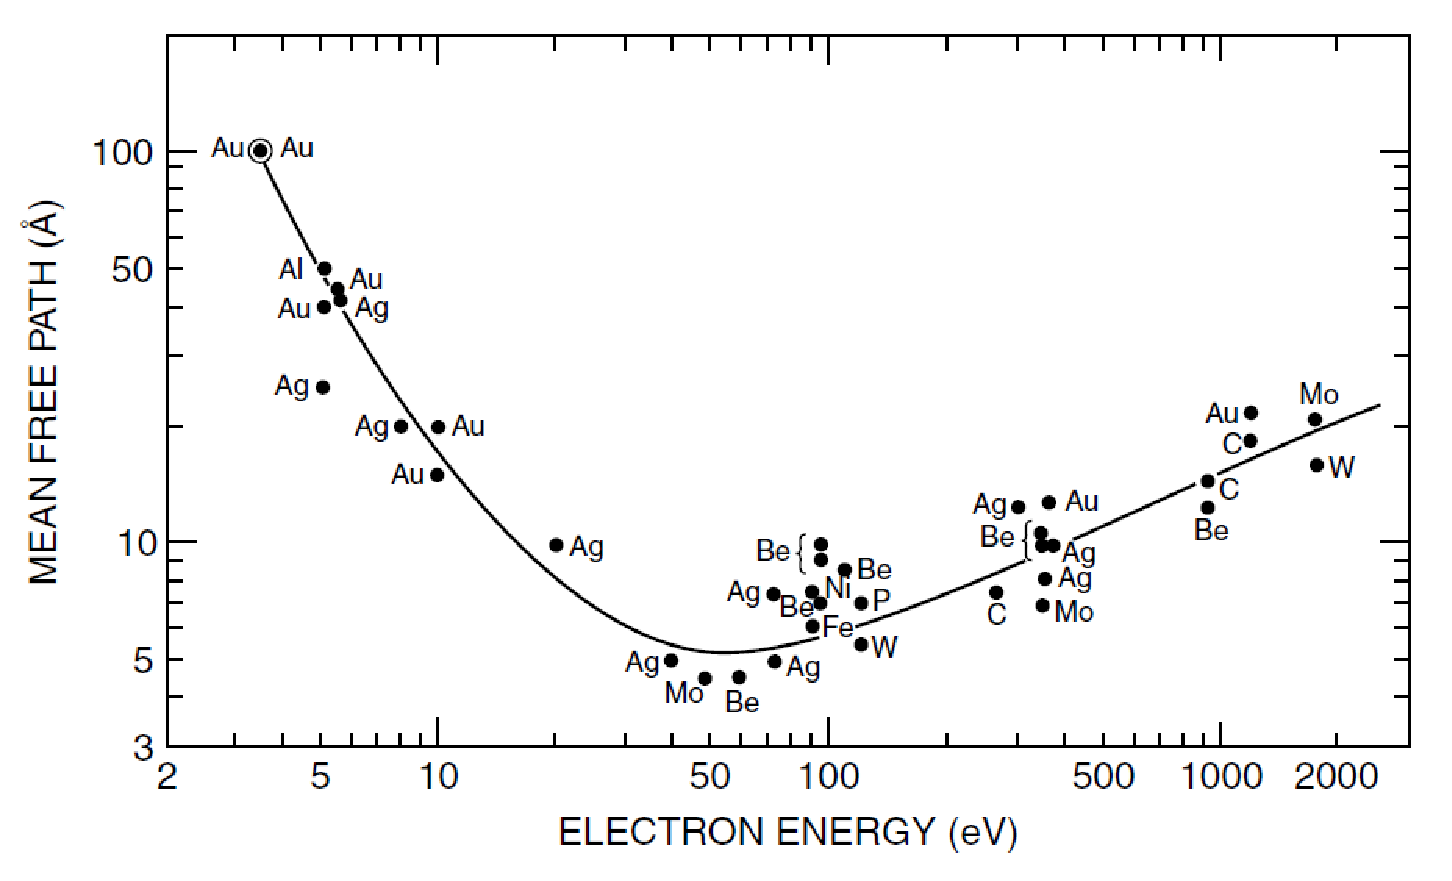
\includegraphics[scale=0.4]{img/ucurve}
\caption{Universal curve of electron escape depth \label{fig:ucurve}}
\end{figure}

\subsection{Inner-Shell Excitations and the Auger Effect}

\begin{figure}
\centering
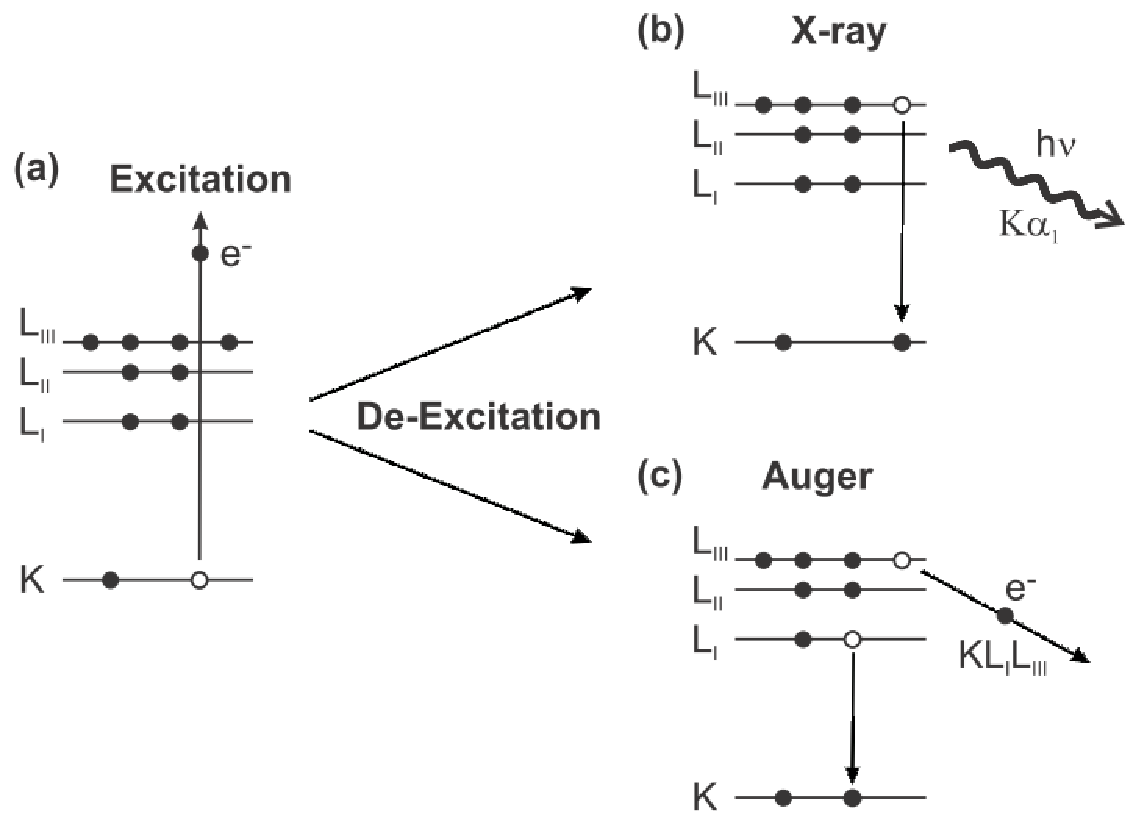
\includegraphics[scale=0.4]{img/auger}
\caption{Auger KLM process \label{fig:aauger}}
\end{figure}


\subsection{Spin-Orbit Coupling}

\begin{equation}
H_{SL} = \Delta H_{T} = - \frac{\mu_B}{0\hbar m_e e c^2}\frac{1}{r}\frac{\partial V(r)}{\partial r} \boldsymbol{L}\cdot\boldsymbol{S}
\end{equation}

\subsection{Plasmons}

\begin{equation}
\omega_{bulk} = \sqrt{\frac{e^2 n}{m_e \epsilon_0}}
\end{equation}

\section{Experimental Setup}

\subsection{Cylindrical Mirror Analyzer}

\begin{figure}
\centering
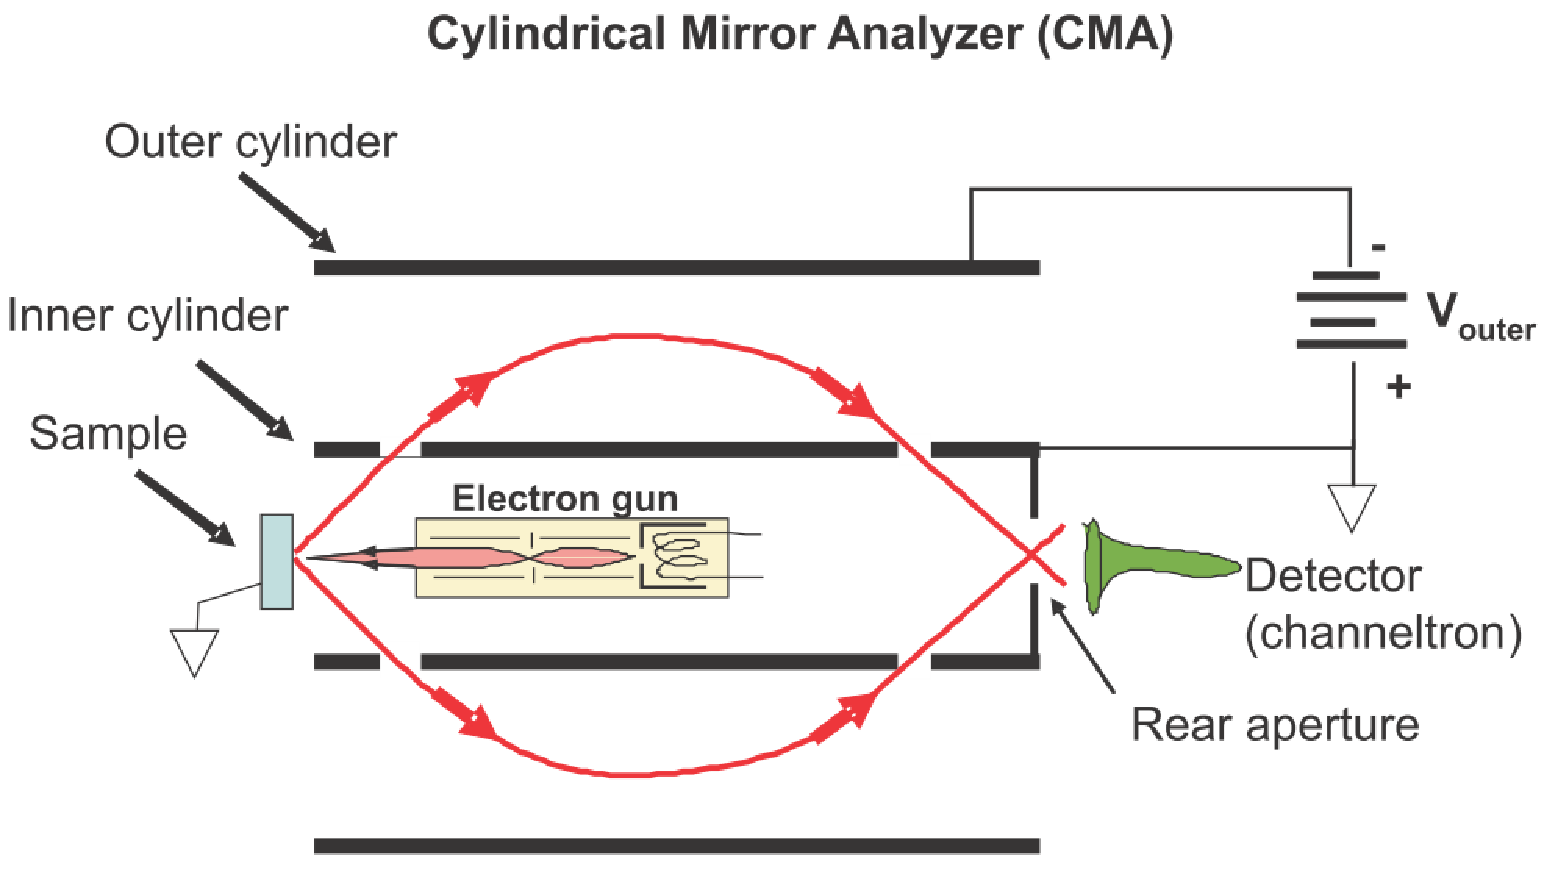
\includegraphics[scale=0.35]{img/cma}
\caption{Cylindrical mirror analyzer \label{fig:cma}}
\end{figure}


\subsection{Channeltron}

\begin{figure}
\centering
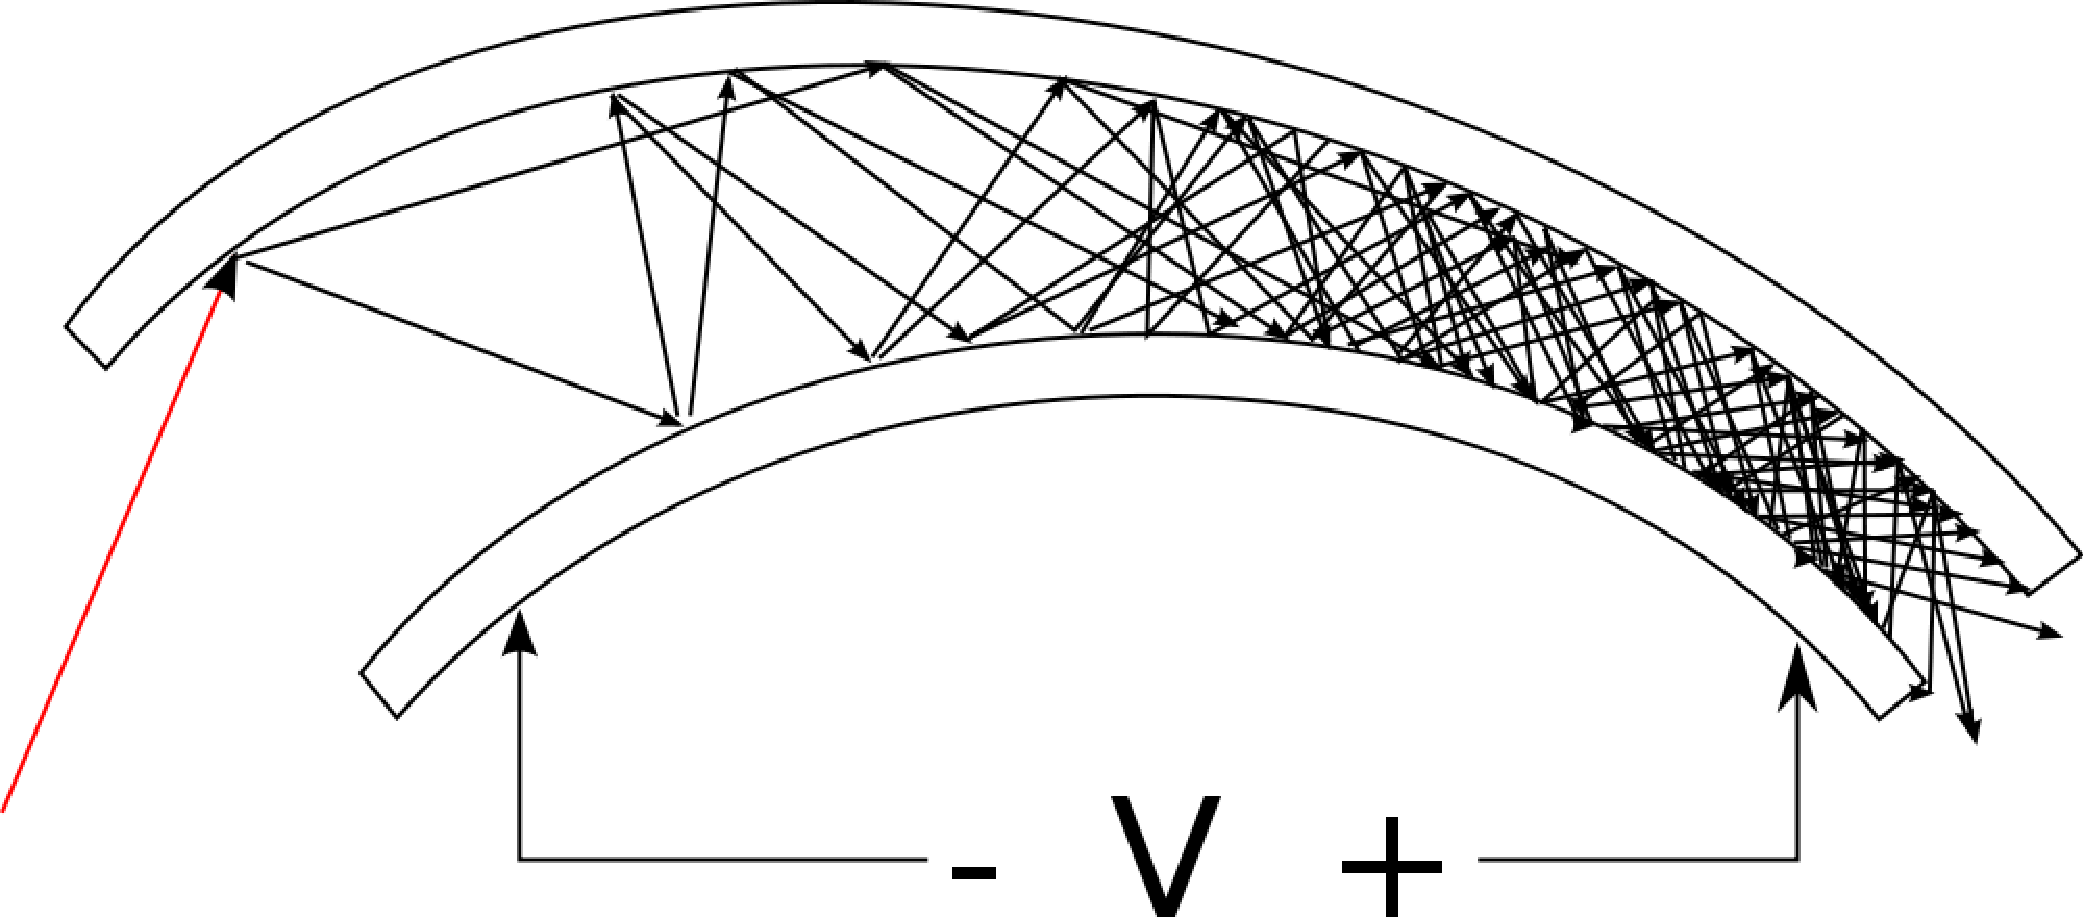
\includegraphics[scale=0.25]{img/channeltron}
\caption{Channeltronh \label{fig:ct}}
\end{figure}


\end{document}
